\chapter{مدل شبکه عصبی و دادگان}

\section{مطاله مقالات جدید}\label{sec1}

در این فصل به مباحث نظری این پروژه کارآموزی اشاره می کنیم. در این فصل بیان می شود که چرا برای این پروژه نیاز به مطاله جدید ترین مقالات حوزه 
بازشناسی گفتار
می‌باشد.
در ادامه بهترین مدل های فعلی 
بازشناسی گفتار
اشاره می شود و خلاصه ای از مقالات آنها بیان می شود ؛
و بعد از مقایسه بهترین مدل های این حوزه بیان می شود که مدل نهایی پروژه 
\texttt{\raggedright E-Branchformer}
 می‌باشد. با استفاده این مدل و دادگان
کامن ویس\LTRfootnote{Common Voice}
 مدل بازشناسی فارسی آموزش داده شده است.
در ادامه به جزئیات دادگان استفاده شده در این پروژه اشاره خواهد شد.
در فصل بعدی به جزئیات پیاده سازی و چالش های آن اشاره خواهد شد.


با توجه به اینکه هدف اصلی این پروژه کارآموزی بروزرسانی مدل فعلی استفاده شده در نرم افزار بازشناسی گفتار فارسی(نویسا) می‌باشد\LTRfootnote{\url{https://nevisalive.com/}}؛ باید جدید ترین مقالات در حوزه بازشناسی گفتار مطالعه شود تا با جدید‌ترین مدل ها و روش های باز‌شناسی گفتار آشنا شد. پس از انجام تحقیقات و مشورت با ارشد پروژه نتیجه این شد که با توجه به اینکه امروزه مدل های 
سر به سر\LTRfootnote{End to End}
بهترین نتایج را دارند از این مدل های استفاده شود. همچنین مدل های ترانسفورمری با دارای بودن خاصیت 
خودنظارتی\LTRfootnote{Self-attention}
در حجم داده های زیاد نتایج بسیار خوبی را خروجی می‌دهند. اخیرا مدل های ترانسفورمری با شبکه های کانولوشنی ترکیب شده اند این امر باعث بهبود قابل توجهی در خروجی آنها شده است.

در مطالعاتی که در این دوره کارآموزی انجام گرفت چند مقاله به منظور یافتن بهترین معماری برای تشخیص گفتار فارسی بررسی شد؛ یکی از بهترین کاندیدا ها مدل \texttt{Whisper} شرکت \texttt{AI Open} می‌باشد. این مدل توانایی بازشناسی گفتار به زبان های مختلف دارد، اما دقت خروجی آن برای زبان فارسی کم است. شرکت عصرگویش پرداز قبلا برای فاین تیون کردن این مدل اقدام کرده است اما با توجه به ماهیت 
نیمه نظارتی
این مدل خروجی مدل فاین توین شده مناسب نبود. با مطالعه و همفکری که در شرکت صورت گرفت تصمیم بر این شد که از مدل های \texttt{Conformer} یا \texttt{Branchformer} برای آموزش مدل بازشناسی گفتار فارسی استفاده شود.

\section{معماری کانفرمر}\label{sec2}
باتوجه به ویژگی های ارزشمند معماری
کانفرمر\LTRfootnote{Conformer}
در این دوره کارآموزی ابتدا مقاله این مدل خوانده شد و گزارشی از آن تهیه شد. در ادامه ویژگی های این مدل و معماری آن را مورد بررسی قرار می دهیم.

اخیراً مدل‌های مبتنی بر شبکه عصبی ترانسفورماتور و کانولوشن 
\LTRfootnote{CNN: Convolutional Neural Network}
نتایج امیدوارکننده‌ای را در تشخیص خودکار گفتار 
بازشناسی گفتار
نشان داده‌اند که عملکرد بهتری از شبکه‌های عصبی بازگشتی 
دارد. مدل‌های ترانسفورماتور در ثبت تعاملات جهانی 
\LTRfootnote{Global Optima}
مبتنی بر محتوا خوب هستند، در حالی که 
\verb;CNN;
ها از ویژگی‌های محلی به طور موثر بهره‌برداری می‌کنند. ترکیب این دو مدل باعث می‌شود که هم ویژگی های محلی و هم جهانی به خوبی استخراج شود. مدل 
کانفرمر
به واسطه معماری خاص خود توانسته است که ویژگی ترانسفورماتور ها و کانولوشن ها را با هم ترکیب کند، و هم در دنباله های کوتاه و بلند داده ها به خوبی عمل کنند. \cite{gulati2020conformer}

معماری مدل کانفورمر
مانند دیگر مدل های سر به سر ترانسفورمری
می‌باشد.
 این مدل از یک بخش
رمزگزار\LTRfootnote{Encoder}
و یک بخش
رمزگشا\LTRfootnote{Decoder}
تشکیل شده است.
این دو بخش توسط جوینت های 
\verb|CTC|
به هم متصل شده اند.
مدل ترانسفورمر در سال 2017 توسط مقاله
\texttt{\raggedright {need you all attention}}
منتشر شد. \cite{DBLP:journals/corr/VaswaniSPUJGKP17}

همین طور که در تصویر 
\ref{fig:transformer}
مشخص است معماری ترانسفورمر ها از بخش های رمزگذار و رمزگشا تشکیل شده است و
تفاوت معماری کانفرمر و ترانسفرمر عادی در ورودی مدل و بخش رمزگذار می‌باشد. در رمزگذار 
 از ترکیب شبکه های کانولوشنی و ترانسفورمری استفاده شده است که این امر این مدل را قادر می سازد درک بهتری از ویژگی های متن ورودی بدست بیاورد.
 
\begin{figure}[H]
  \centering
  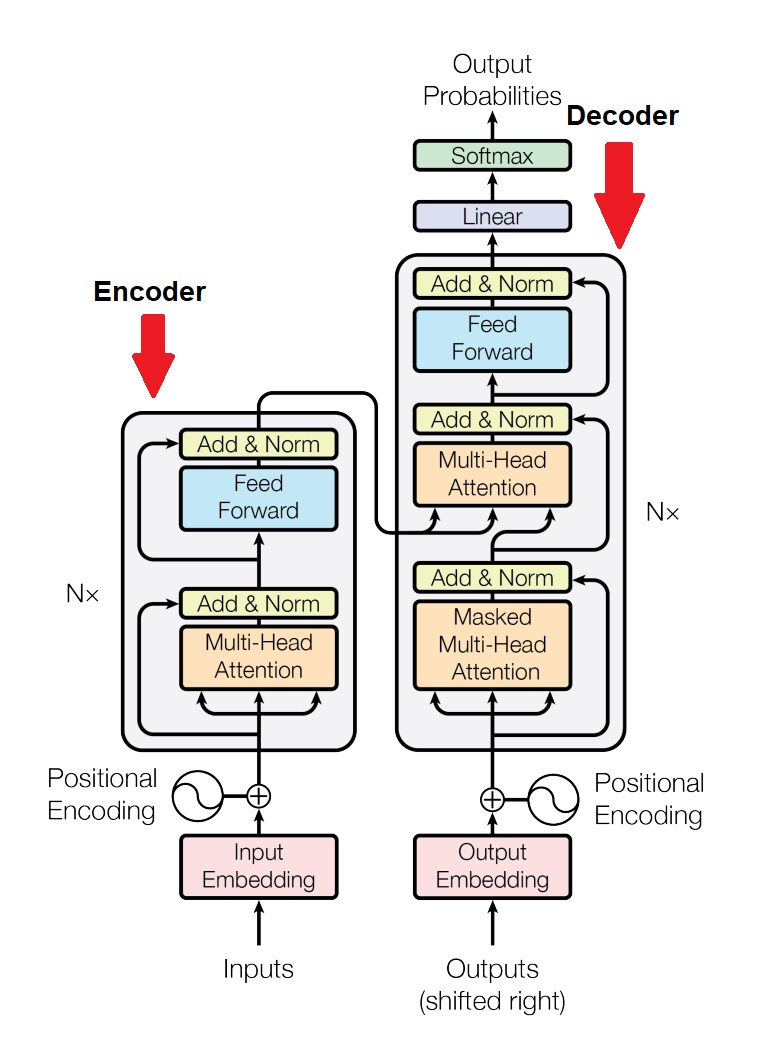
\includegraphics[width=0.6\textwidth, height=13cm]{Images/Chapter2/transformer.jpg}
  \caption{تصویر معماری مدل ترانسفورمر. این مدل از یک بخش رمزگذار و رمزگشا تشکیل شده است و بخش های آن توسط فلش در تصویر مشخص است.}
  \label{fig:transformer}
\end{figure}

 همان طور که از تصویر \ref{fig:conformer}
مشخص است.
بلاک کانقرمر یک ماژول 
  \verb|Forward Feed|
  و بعد از آن ماژول 
  خود نظارتی
  آمده است.
  سپس خروجی این ماژول وارد ماژول  کانولوشن می شوند
  در نهایت نیمی از ابعاد  وارد 
  \verb|Forward Feed|
  می شود.
  در مرحله آخر یک بلوک 
  \verb|Layernorm|
  قرار داده شده است.
  
 \begin{figure}[H]
  \centering
  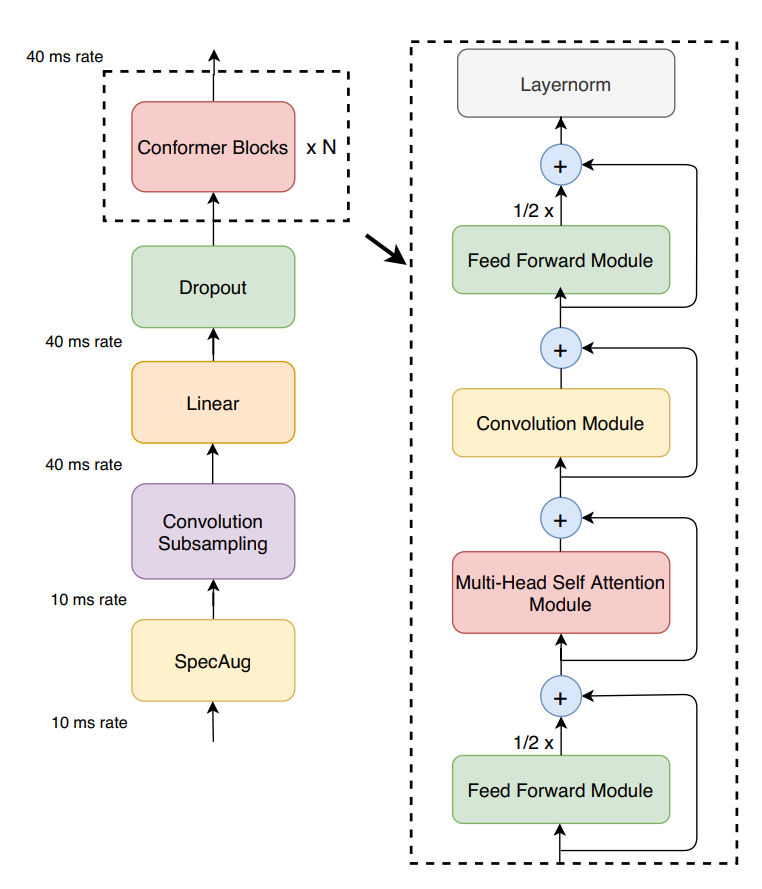
\includegraphics[width=0.5\textwidth,height=9cm]{Images/Chapter2/conformer.png}
  \caption{
  معماری رمزگذار کانفرمر. 
  }
  \label{fig:conformer}
\end{figure}



همان طور که پیش تر گفته شد این امر معماری کانفرمر را قادر می سازد که هم ویژگی های جهانی و هم ویژگی های محلی را به خوبی تشخیص بدهد. این معماری عالی معماری کانفرمر را به یکی از بهترین مدل های موجود برای کار های 
بازشناسی گفتار
تبدیل کرده است.
این مدل یکی از بهترین کاندیدا های مدل 
بازشناسی گفتار فارسی
بود. من در این دوره کارآموزی مقاله کانفرمر را مطاله کردم و چند پیاده سازی از آن را بررسی کردم. مقاله خوانده شده در یک جلسه برای اعضای بخش تحقیقات و توسعه\LTRfootnote{Research and Development} شرکت معرفی شد و نظرات آنها در مورد این مدل دریافت شد.
این مدل با تمام ویژگی های خوب آن اندکی قدیمی شده است و مدل های جدید تر وجود دارند که ادعا می کنند به نتایج بهتری دست یافته اند.
در بخش بعدی به یکی از بهترین آنها اشاره می شود.

\section{معماری ای-برانچفرمر}
یکی از جدید ترین معماری های ارائه شده در حوزه 
بازشناسی گفتار
معماری 
ای-برانچفرمر\LTRfootnote{E-Branchformer}
می‌باشد.

این مدل که در کنفراس
\verb|Interspeech|
سال 2023
معرفی شد و نتایج خوبی که بر روی دیتاست های مختلف بدست آورد توجه های زیادی را بخودش جلب کرده است.

مدل
\texttt{\raggedright E-Branchformer}
بهبود یافته مدل 
\texttt{\raggedright Branchformer}
می‌باشد.\cite{kim2022ebranchformer}
حرف 
\verb|E|
مخفف کلمه
\verb|Enhanced|
می‌باشد که به معنای تقویت شده می‌باشد و ای-برانچفرمر تقویت شده مدل برانچفرمر می‌باشد.
برانچفرمر های ساختاری بسیار مشابه به کانفرمر ها دارند. در برانچفرمر ها نیز فقط معماری بخش رمزگذار با  معماری ترانسفر ها متفاوت است، در رمزگذار آن مانند کانفرمر ترکیبی از بلوک های کانفرمری و 
خود نظارتی
استفاده می شود تا هم ویژگی های محلی و هم جهانی داده ها به خوبی توسط مدل درک شود.

تفاوت اصلی کانفرمر و برانچفرمر در نوع ترکیب بلوک های 
کانفرمری و 
خود نظارتی
می‌باشد.
در برانچفمر ها تلاش شده است که این ترکیب به صورت موازی انجام شود، در حالی که در کانفرمر این ترکیب به صورت سری انجام شده است این امر در شکل \ref{fig:conformer} مشخص است. 
موازی سازی انجام شده در برانچفرمر ها باعث می شود که عمق شبکه عصبی کمتر شود و راحت تر به نقطه بهینه همگرا شود.
همچنین تعداد پارامتر های استفاده شده در برانچفرمر در تعداد لایه های برابر کمتر از کانفرمر ها می‌باشد، که امر باعث کاهش هزنیه محاسباتی آموزش این مدل می شود.

 \begin{figure}[H]
  \centering
  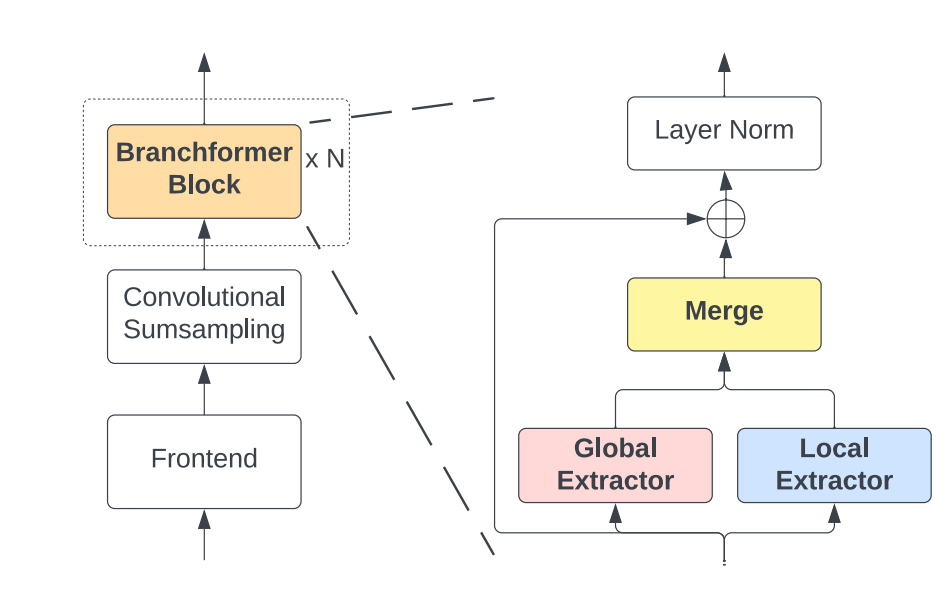
\includegraphics[height=6cm]{Images/Chapter2/EBranchformer.png}
  \caption{
  معماری رمزگذار برانچفرمر.
  }
  \label{fig:EBranchformer}
\end{figure}

شکل \ref{fig:EBranchformer}
معماری رمزگذار برانچفرمر را نمایش می دهد. همین طور که مشخص است نیمی از ابعاد داده ها به استخراج کننده محلی\LTRfootnote{Local} و نیم دیگر به استخراج کننده جهانی داده می شود. این نوع معماری خاص مدل را قادر می سازد که هم ویژگی های محلی و هم ویژگی های جهانی\LTRfootnote{Global} را به خوبی تشخیص دهد و مدل هم در دنباله\LTRfootnote{Sequence} داده های کوتاه و هم در دنباله داده های بلند خوب عمل کند.

تفاوت 
برانچفرمر
و
ای-برانچفرمر
این نوع ترکیب این دو بخش موازی می‌باشد.
ای-برانچفرمر بسیار بهینه تر با این دو بخش را باهم ترکیب می‌کند.
در ادامه برای یافتن بهترین مدل برای 
بازشناسی گفتار
باید مطالعه ای صورت بپذیرد که بهترین مدل ممکن برای آموزش استفاده شود.
در بخش بعدی به مطالعه مقاله ای پرداخته می شود که این دو مدل برتر یعنی ای-برانچفرمر و کانفرمر را با هم مقایسه کرده است و بهترین مدل را معرفی کرده است.



\section{مقایسه ای-برانچفرمر و کانفرمر}\label{sec4}

اخیرا مقاله ای چاپ در چاپ شده است که دو مدل برتر ای-برانچفرمر و کانفرمر را باهم مقایسه می‌کند.\cite{peng2023comparative}
این مقاله این دو مدل را در سه تا از تسک های گفتار بازشناسی گفتار، ترجمه گفتار و درک گفتار بررسی می‌کند. مقایسه در تعدادی از بزرگترین و معروف ترین دیتاست های منبع باز صورت گرفته است؛ و خروجی های این مدل ها بر روی این دیتاست ها با هم مقایسه شده اند.

 \begin{figure}[H]
  \centering
  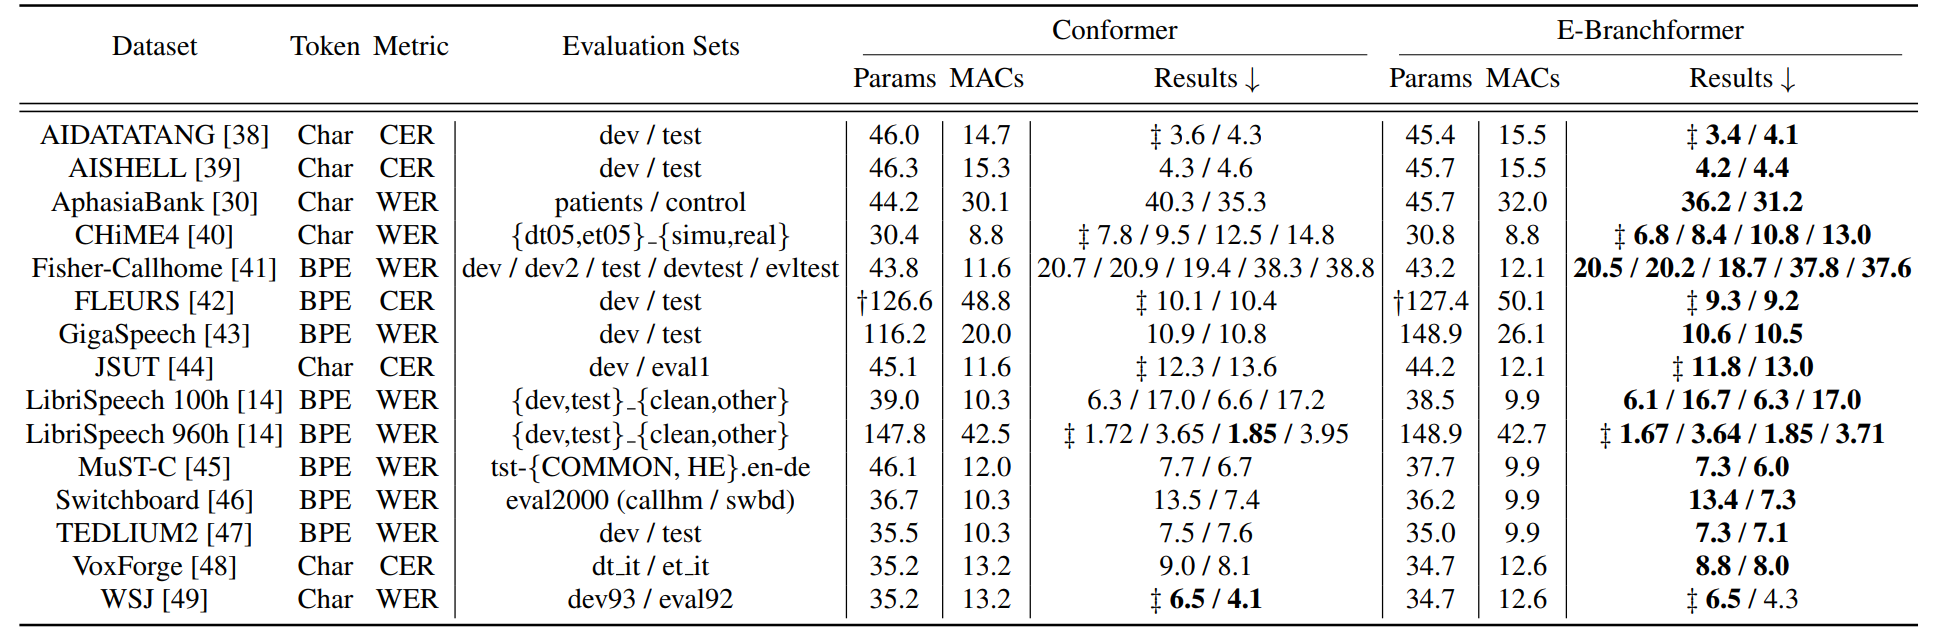
\includegraphics[width=1\textwidth,height=6cm]{Images/Chapter2/confvsbranch.png}
  \caption{
  جدول مقایسه کننده دو مدل کانفرمر و ای-برانچفرمر. این دو مدل در 12 دیتاست با هم مقایسه شده اند.
  }
  \label{fig:confvsbranch}
\end{figure}

همین طور که در تصویر \ref{fig:confvsbranch}
مشخص است مدل ای-برانچفرمر نتایج بسیار بهتری نسبت به کانفرمر در اکثر دادگان بدست آورده است.
این جدول و جداول دیگری که در این دو مدل را در تسک های مختلف مقایسه می کنند نشان می‌دهند که مدل ای-برانچفرمر نتایج بسیار بهتری نسبت به کانفرمر در هر سه تسک گفتار بدست آورده است. این مقاله بر برتری ای-برانچفرمر تأکید می‌کند زیرا معماری موازی شده رمزگذار آن باعث بهبود نتایج و کاهش هزینه محاسباتی شده است.

با توجه به نتایج بهتر مدل ای-برانچفرمر بعد از مشورت هایی که در گروه انجام شد تصمیم بر این شد که این مدل برای بازشانسی گفتار فارسی استفاده شود و این مدل بر روی دادگان فارسی آموزش داده شود و خروجی آن بررسی شود.
این مقاله همچنین اشاره شده است که از ابزار
\verb|ESPnet|
برای آموزش دو مدل کانفرمر و ای-برانچفرمر بر روی دادگان مختلف استفاده شده است و دستورعمل های
\LTRfootnote{Recipe} دستور عمل ها
پیشفرض آن در آموزش استفاده شده است.
جعبه ابزار\LTRfootnote{Toolkit} یی-اس-پی نت\LTRfootnote{ESPnet} ابزاری بسیار قدرتمند در ضمیه بازشناسی گفتار می‌باشد
و کاربرد گسترده آن در تسک های مختلف گفتار و ارجاعات زیاد در مقالات جدید، فراگیری این ابزار برای ادامه کار الزامی می‌باشد. در فصل بعدی به یادگیری این ابزار و چالش های پیاده سازی با آن اشاره شده است.


\section{دادگان}\label{sec5}
بر اساس پیشنهاد ارشد پروژه تصمیم بر این شد که که مدل ابتدا بر رو دادگان پایگاه داده 
\verb|Voice Common|
آموزش داده شود و خروجی مدل بررسی شود.
در شرکت عصر گویش پرداز مدل های قبلی 
بازشناسی گفتار
ابتدا بر روی این دادگان آموزش داده شده اند؛ آموزش بر روی دادگان این امکان را فراهم می‌کند که نتایج خروجی این مدل با مدل های قدیمی شرکت مقایسه شود. این پایگاه داده زبان فارسی را هم پشتیبانی می‌کند و داده های مورد نیاز برای بازشناسی گفتار فارسی را دارا می‌باشد. در ادامه جزئیات این پایگاه داده بیان می شود.

کامن ویس\LTRfootnote{Common Voice}
یک پروژه جمع سپاری است که توسط شرکت موزیلا برای ایجاد یک پایگاه داده رایگان برای نرم افزار تشخیص گفتار آغاز شده است. این پروژه توسط داوطلبانی پشتیبانی می شود که جملات نمونه را با میکروفون ضبط می کنند و ضبط های دیگر کاربران را بررسی می کنند. جملات بازشناسی شده در یک پایگاه داده صوتی که تحت مجوز مالکیت عمومی
\verb|CC0|
در دسترس است، جمع آوری می شود. این مجوز تضمین می‌کند که توسعه دهندگان می توانند از پایگاه داده برای برنامه های صوتی به متن بدون محدودیت یا هزینه استفاده کنند.

این پایگاه داده دارای داده صوتی و متنی از 112 تا زبان های دینا می‌باشد و مجموعاً 28 هزار ساعت داده در این پایگاه داده موجود است. داده های این پایگاه داده برای عموم مردم به راحتی در سایت این پایگاه داده در دسترس است.\LTRfootnote{ https://commonvoice.mozilla.org/}
در آخرین نسخه حال حاظر این دادگان برای زبان فارسی 397 ساعت داده صوتی به همراه متن متناظر با آن موجود می‌باشد. البته فرمت فایل های صوتی 
\verb|mp3|
می‌باشد که این فرمت برای پردازش در مدل های گفتاری مناسب نمی‌باشد و باید فرمت آن تغییر کند این خود یکی از چالش هایی بود که من در این پروژه با آن مواجه شدم که در فصل بعد به جزئیات آن اشاره خواهد شد. یکی از مشکلات این پایگاه داده این است که درستی تطابق همه داده های صوت و متن بررسی نشده است و فقط بخشی از داده ها توسط کابران بررسی شده است. با این حال بعد از بررسی که از این پایگاه داده انجام گرفت به این نتیجه رسیدیم که اکثر داده ها تطابق خوبی دارند و این پایگاه داده برای آموزش نسخه های اولیه مدل بازشناسی گفتار فارسی مناسب می‌باشد.

در ادامه از این پایگاه داده برای آموزش دادن مدل بازشناسی گفتار فارسی با معماری ای-برانچفرمر استفاده شده است و از ابزار
\verb|ESPnet|
به این منظور مورد استفاده قرار گرفته شده است. در فصل بعدی به پیاده سازی عملی این پروژه کارآموزی و چالش های آن اشاره خواهیم کرد.

